\begin{figure}[H]
	\centering
	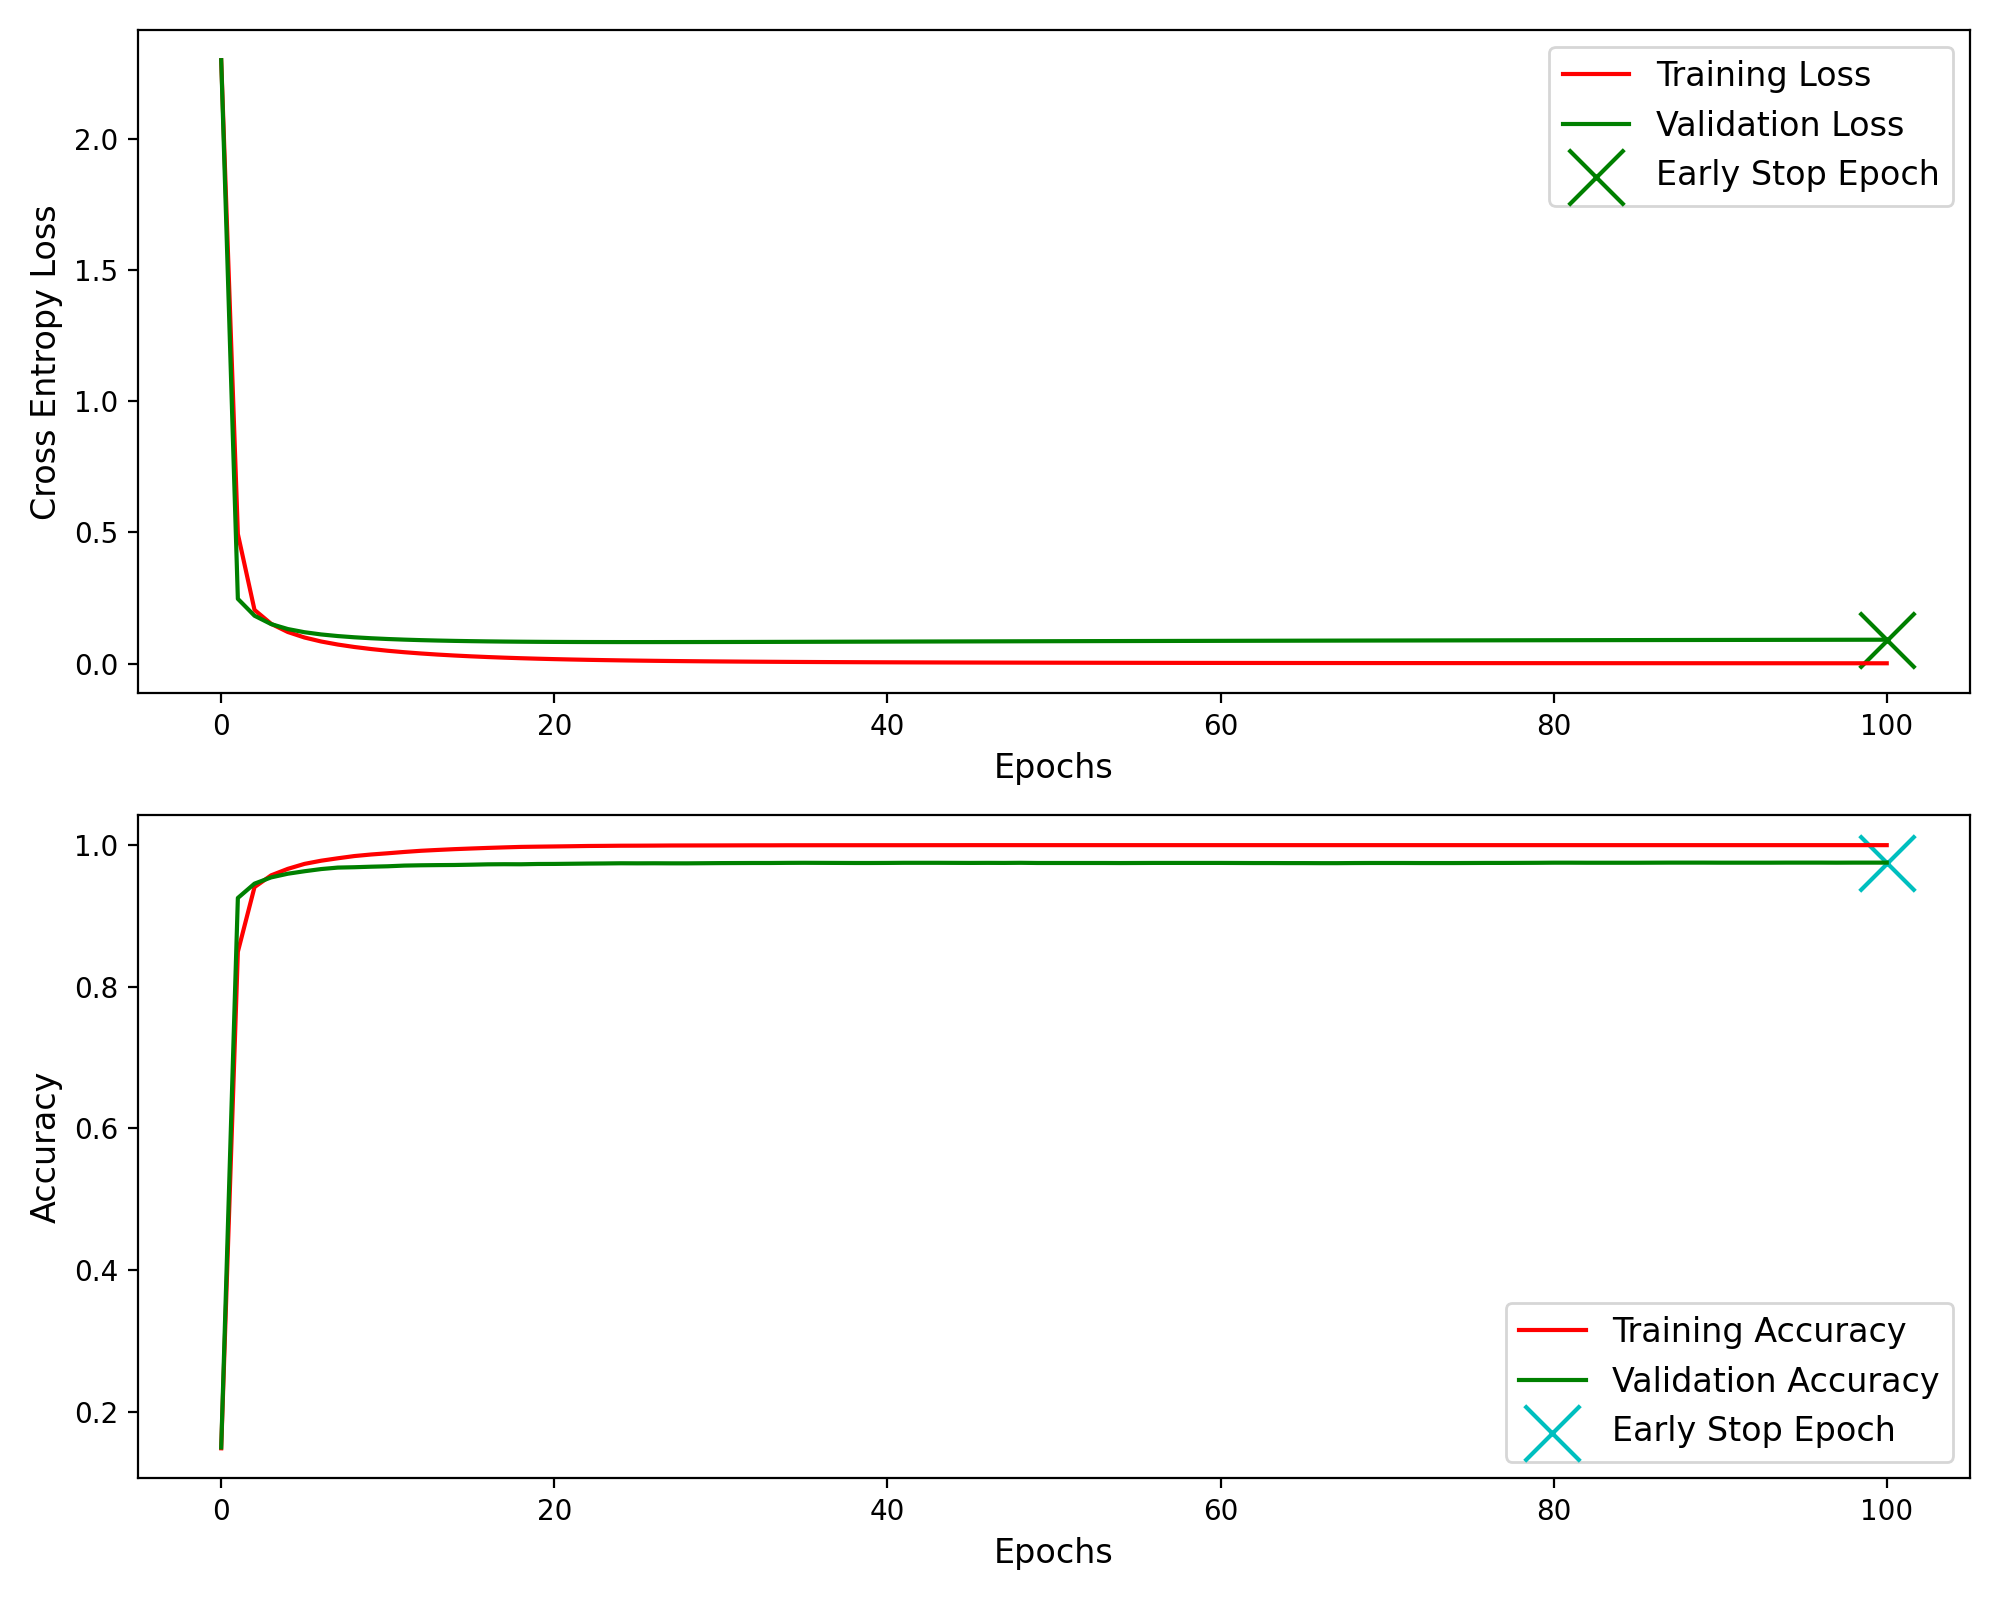
\includegraphics[width=1.0\textwidth]{./images/no_momentum_no_early_stop.png}
	\caption{Accuracy and Loss without momentum or early stopping}
	\label{fig:no_momentum_no_early_stop}
\end{figure}
\begin{figure}[H]
	\centering
	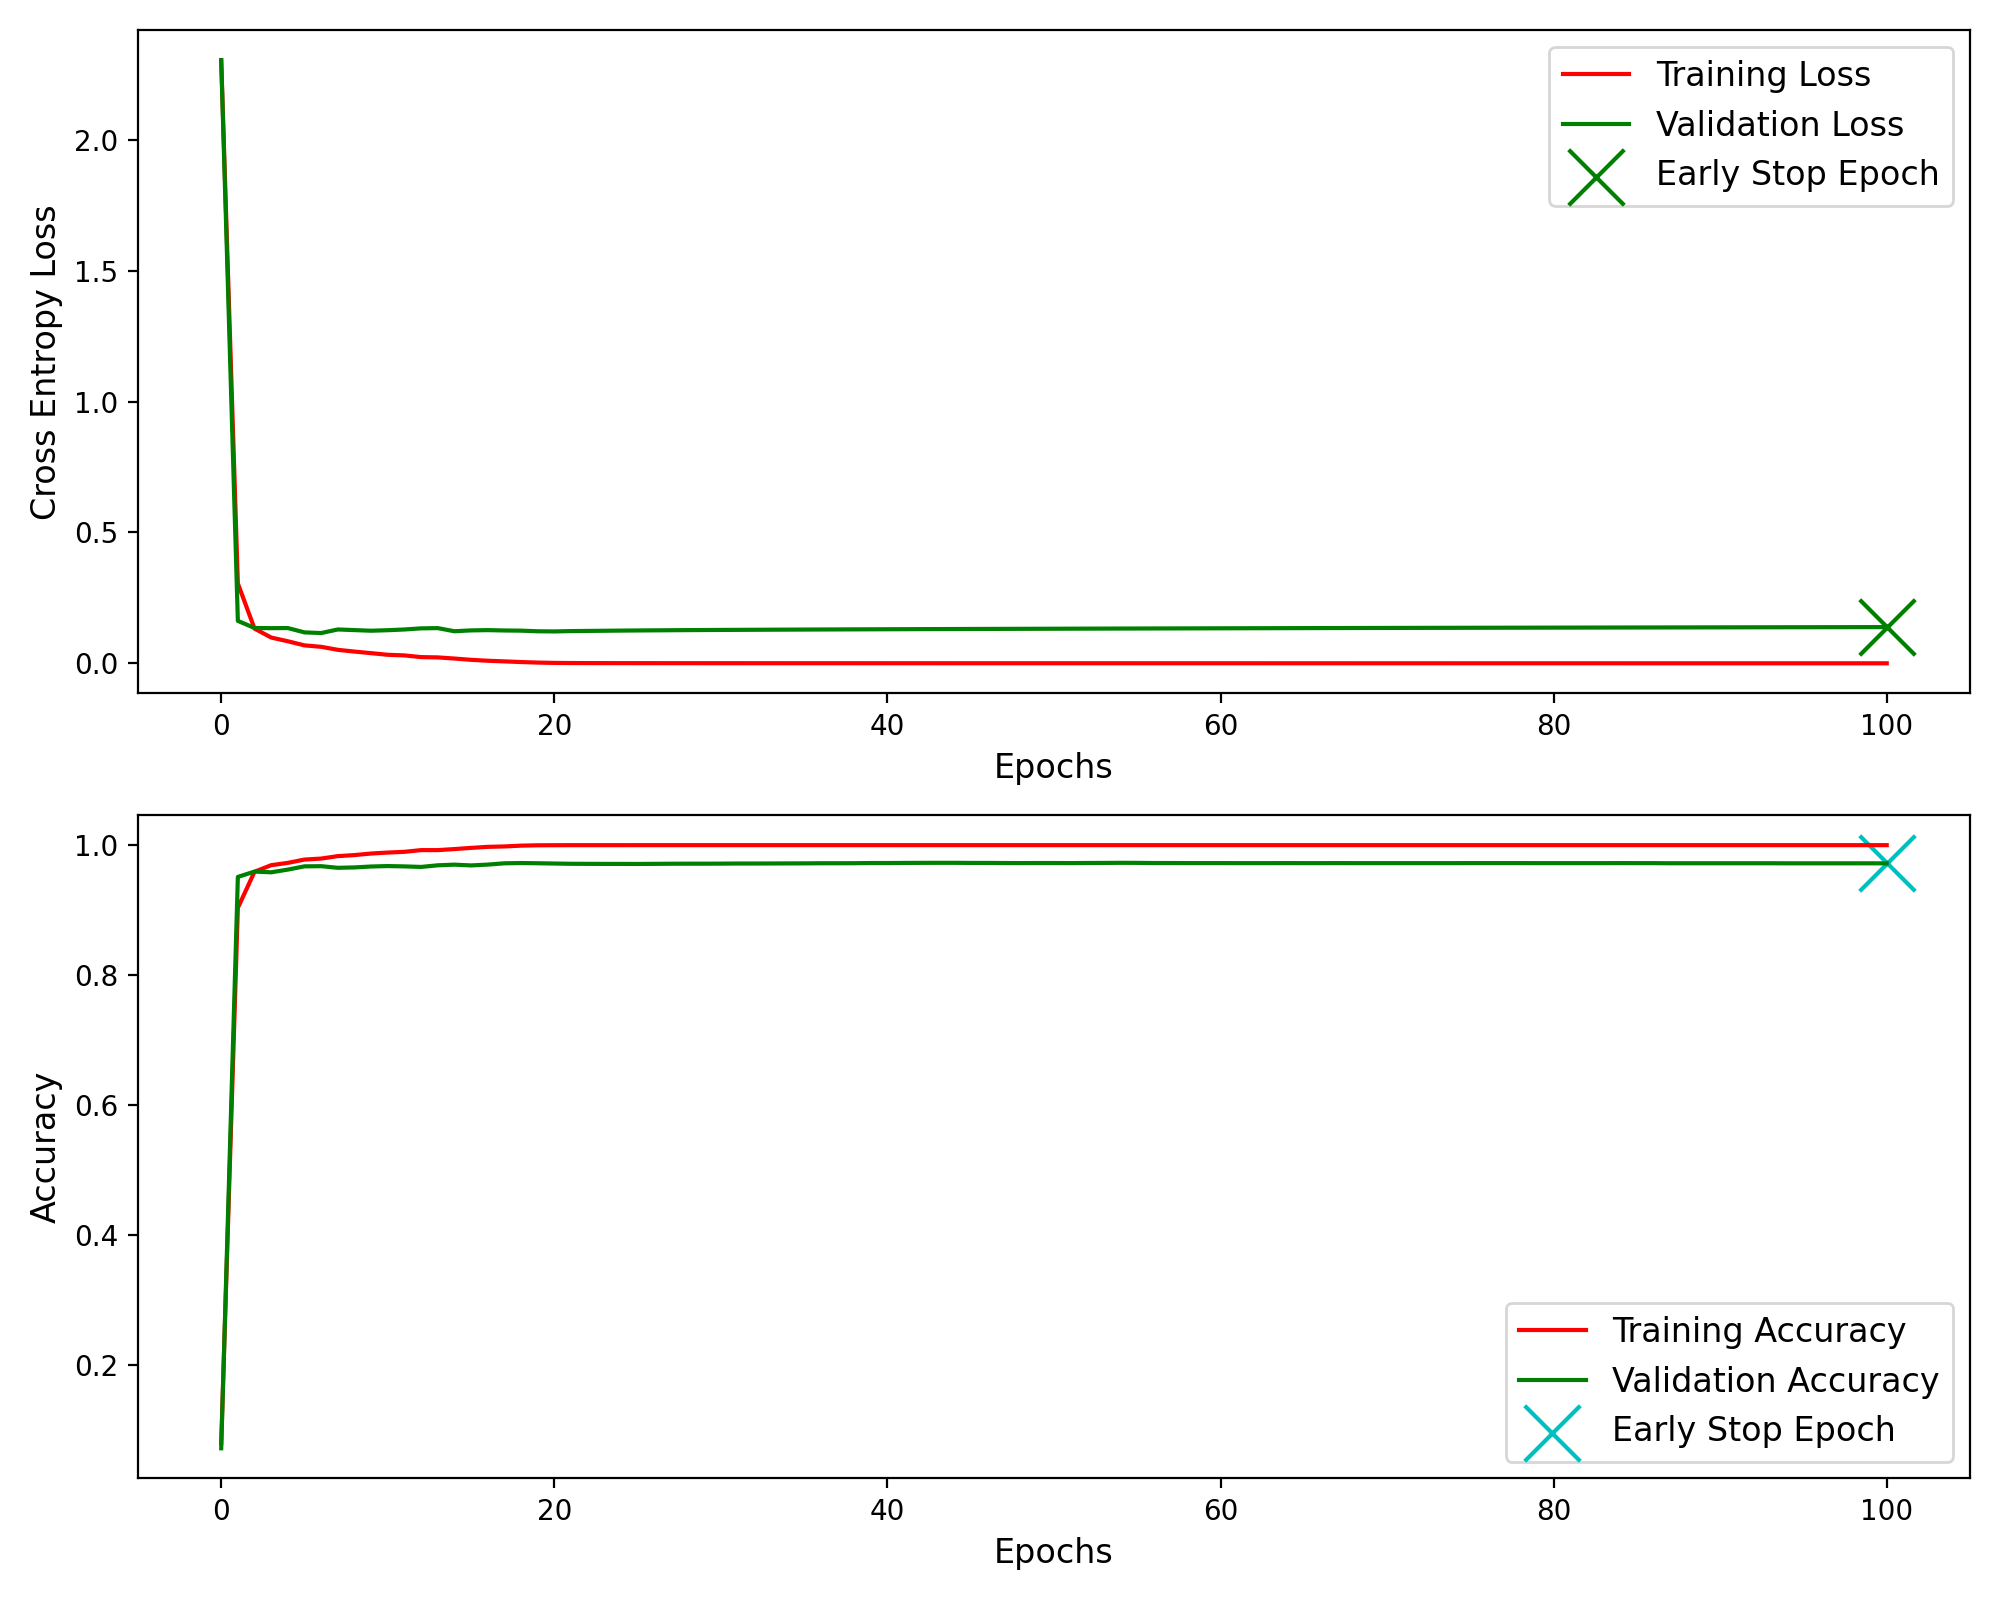
\includegraphics[width=1.0\textwidth]{./images/momentum_no_early_stop.png}
	\caption{Accuracy and Loss with momentum and without early stopping}
	\label{fig:momentum_no_early_stop}
\end{figure}

\begin{figure}[H]
	\centering
	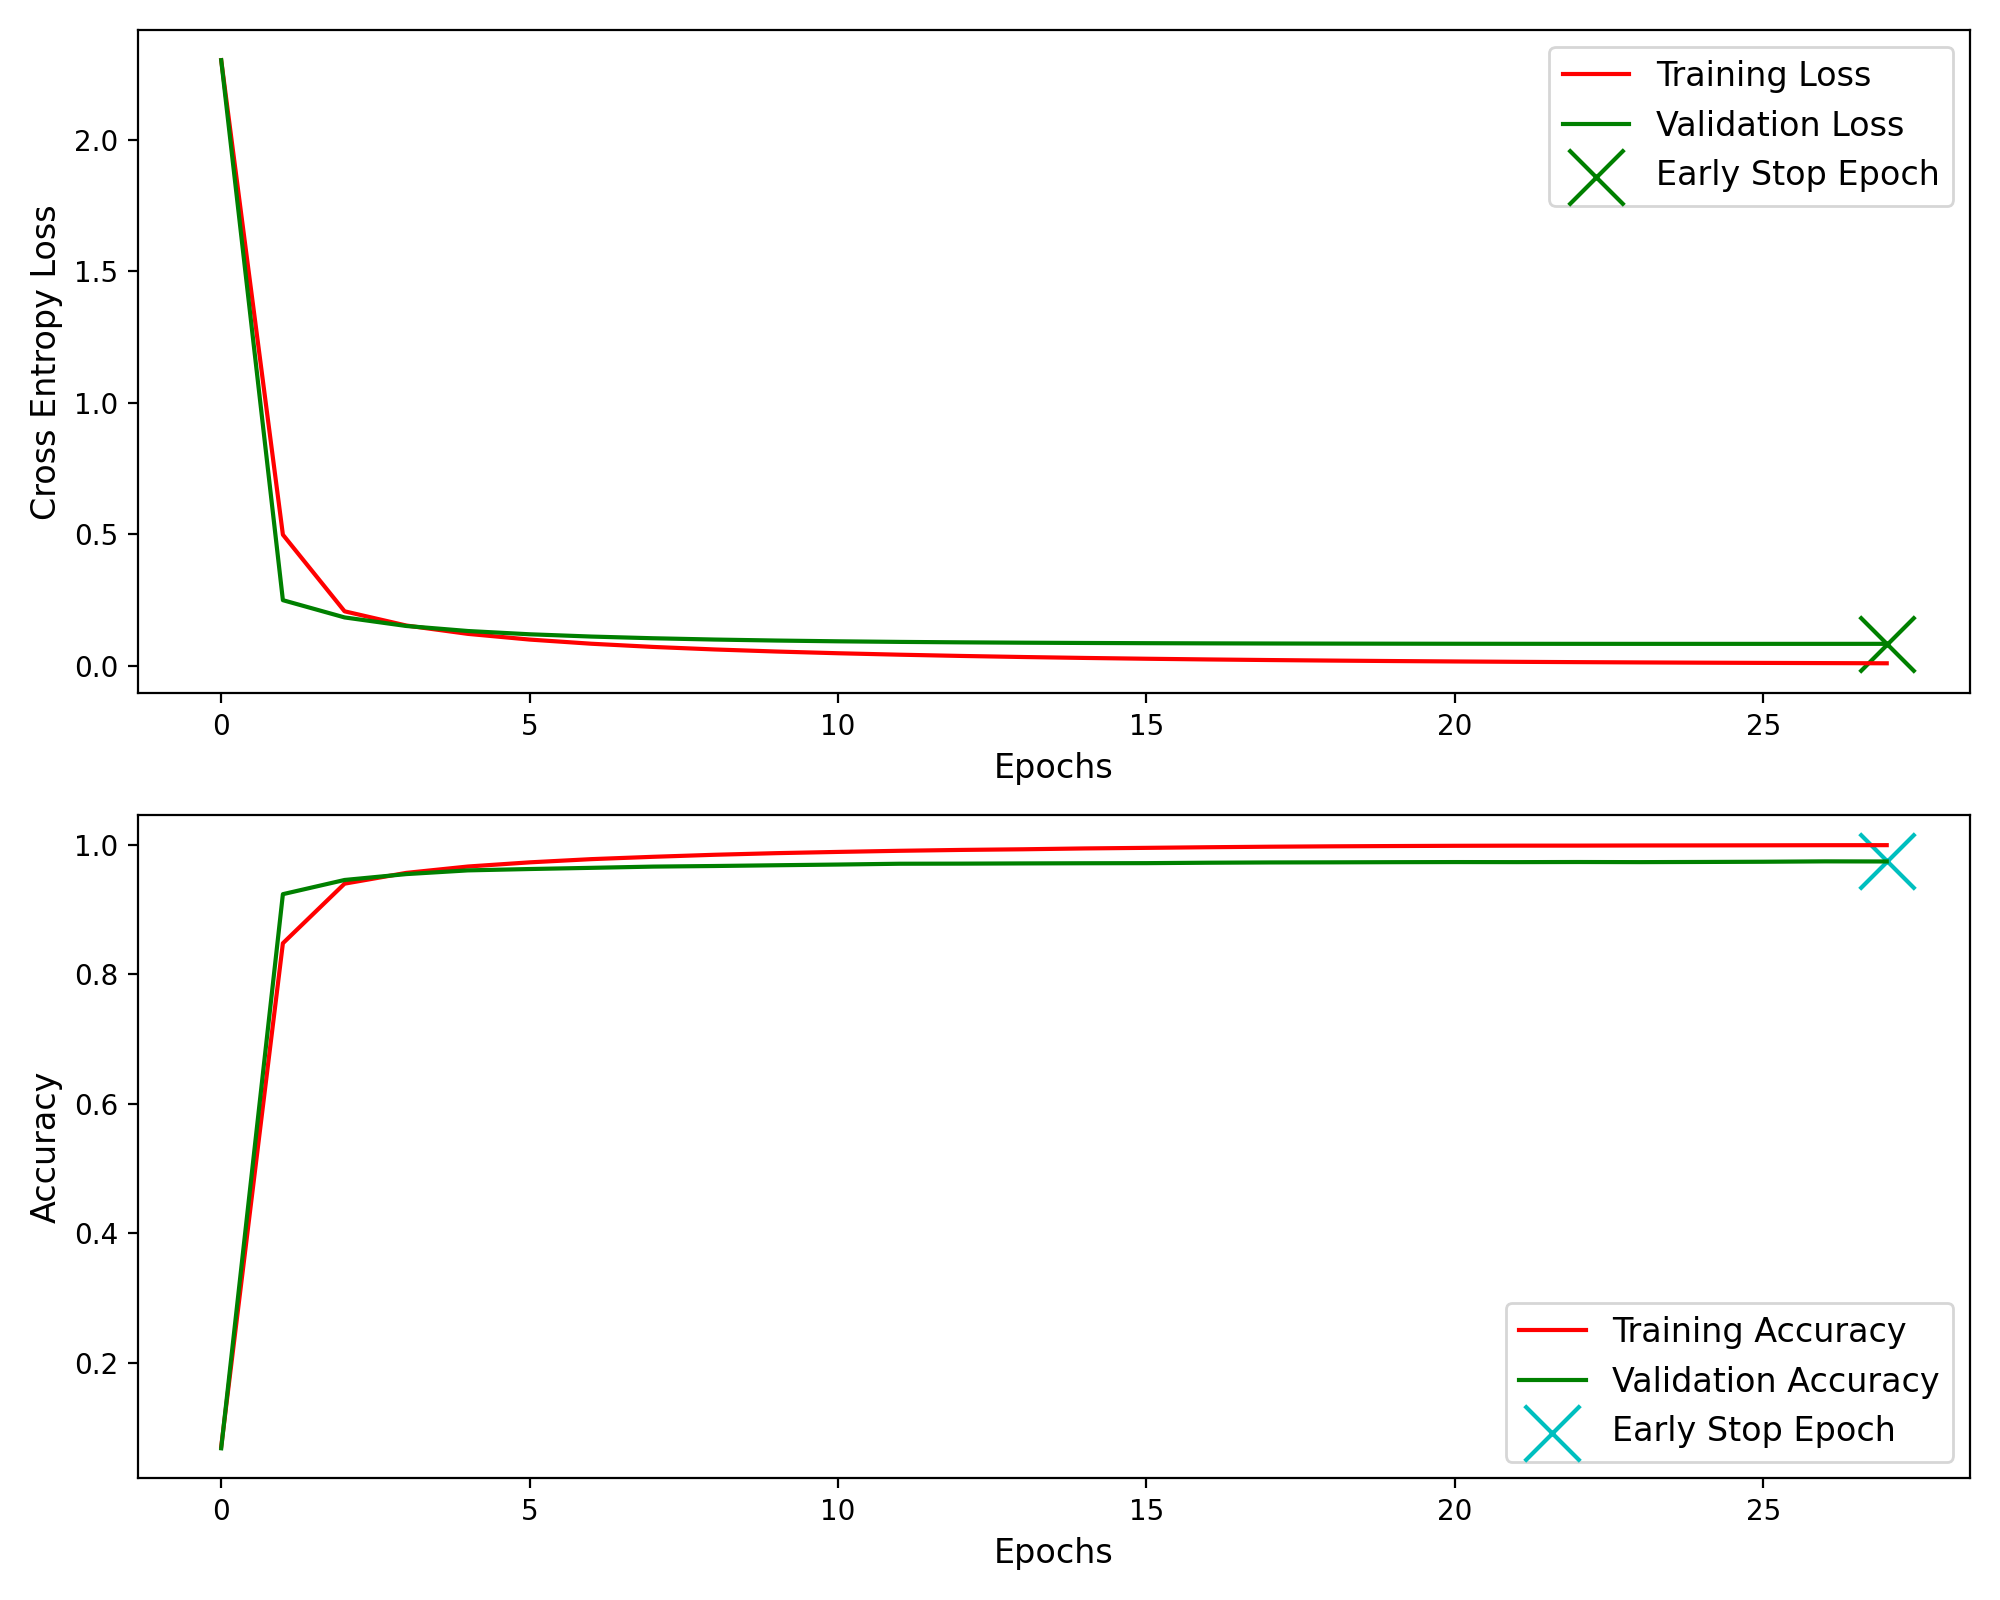
\includegraphics[width=1.0\textwidth]{./images/early_stop_no_momentum.png}
	\caption{Accuracy and Loss with early stopping and without momentum}
	\label{fig:early_stop_no_momentum}
\end{figure}


\begin{figure}[H]
	\centering
	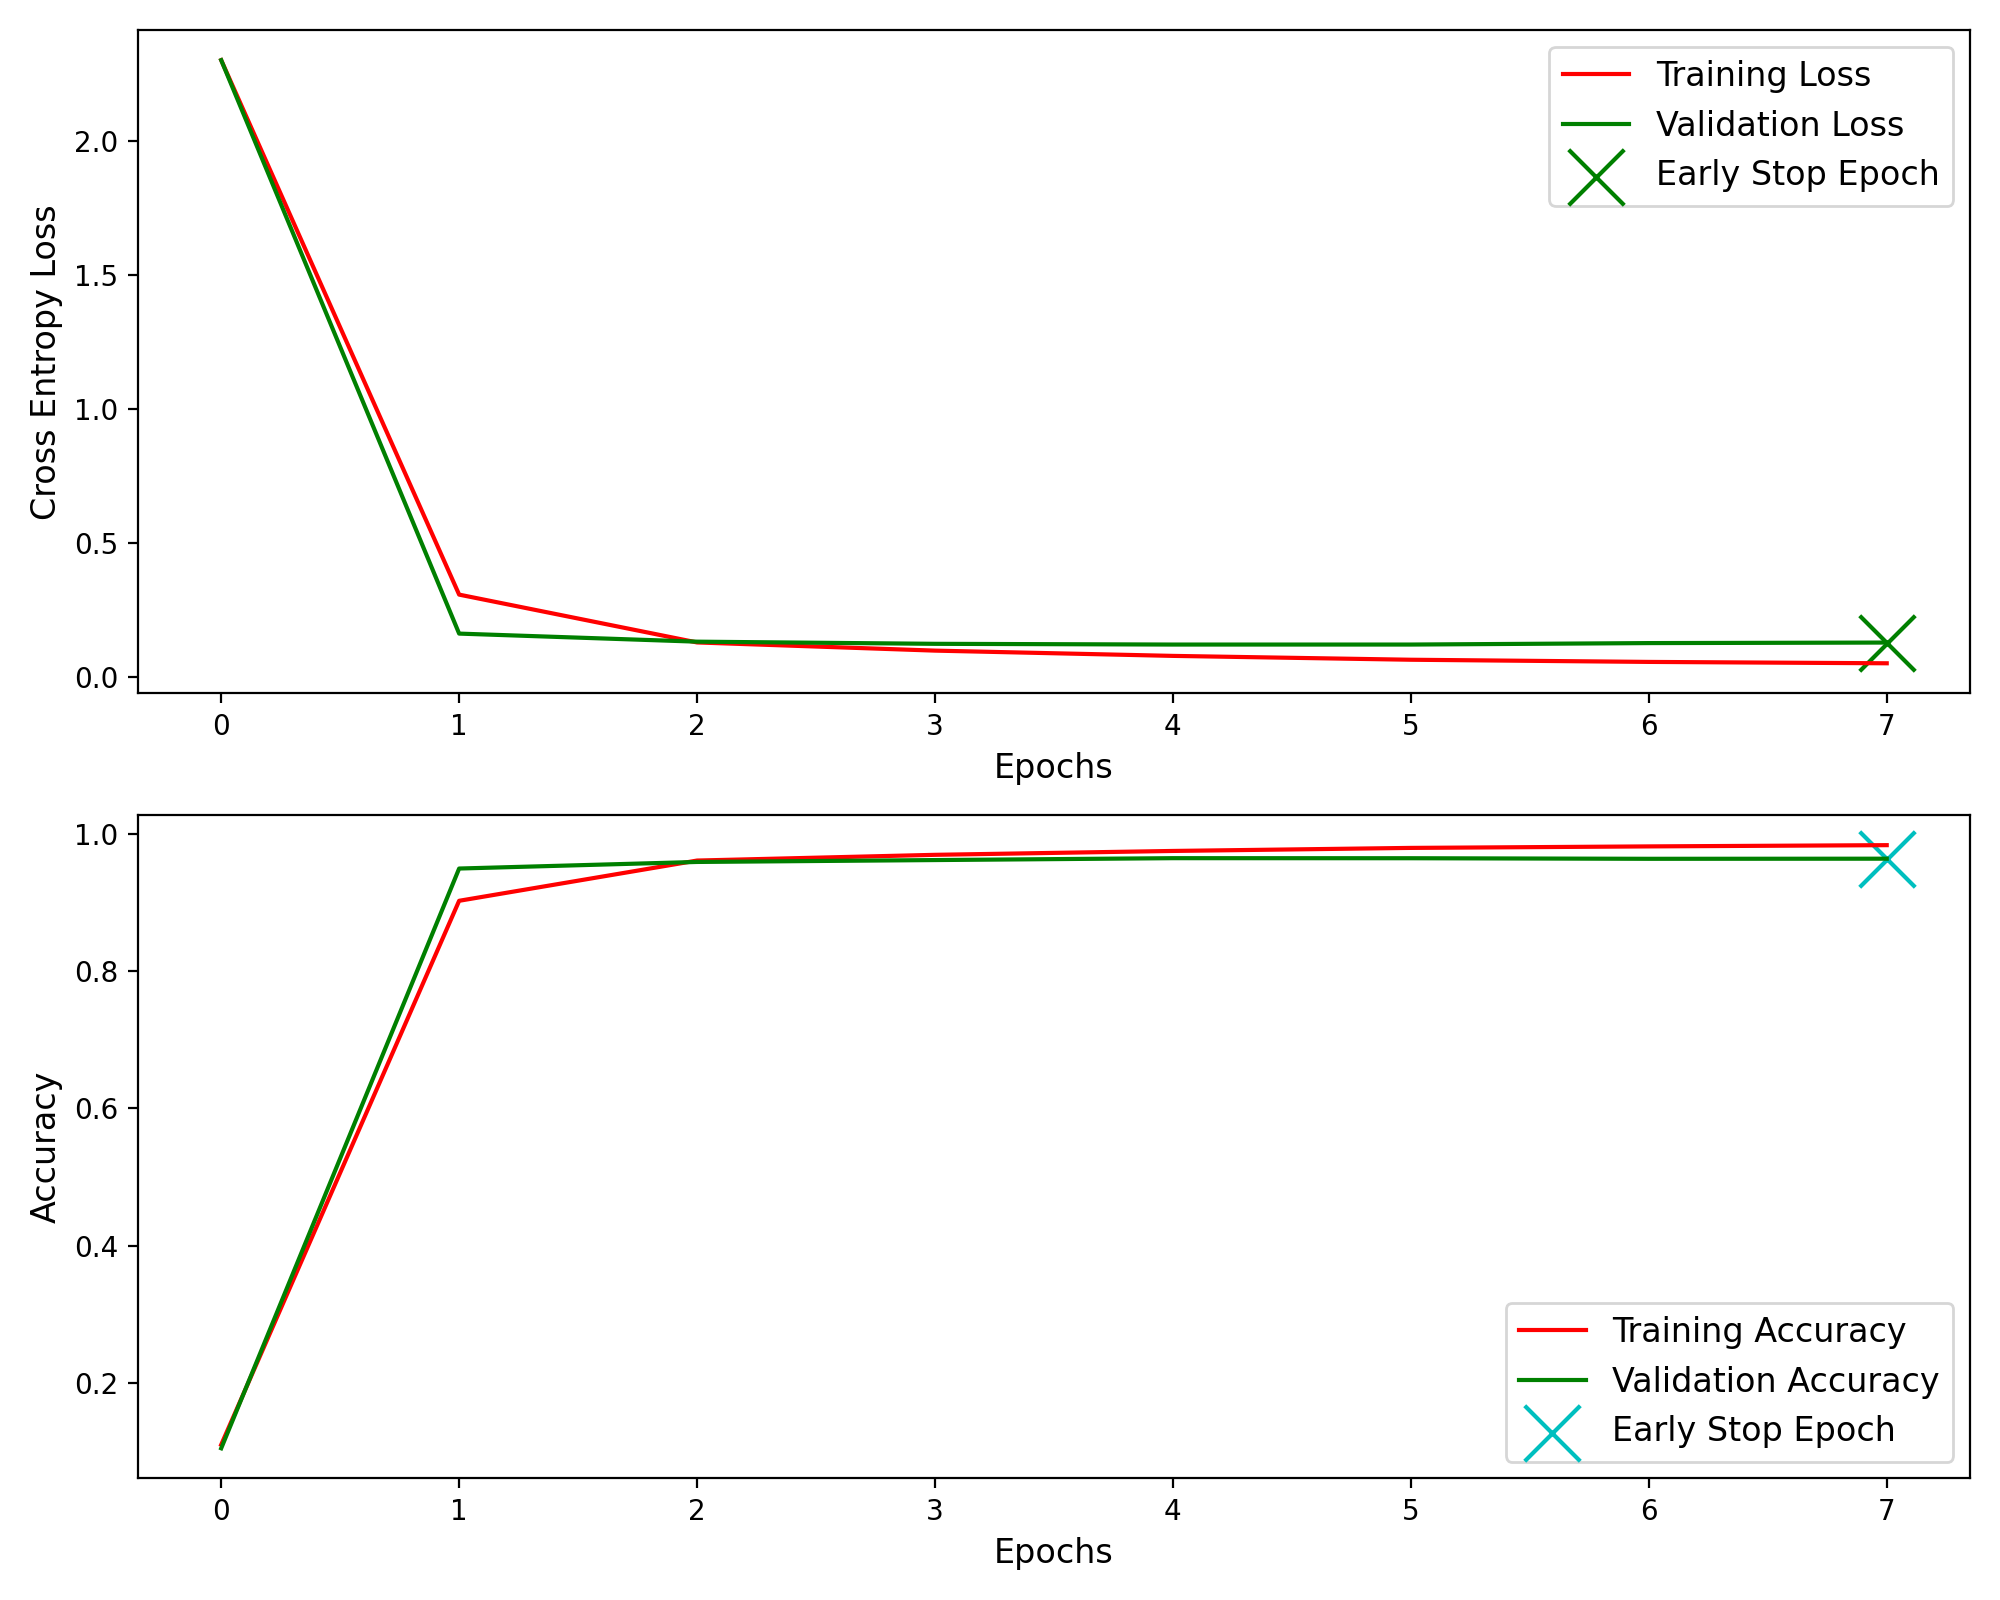
\includegraphics[width=1.0\textwidth]{./images/momentum_early_stop.png}
	\caption{Accuracy and Loss with early stopping and momentum}
	\label{fig:momentum_early_stop}
\end{figure}

\section{Momentum Experiments}

\subsection{Background}

We now consider a new network with a 785 neuron input layer, a 128 neuron
hidden layer, and a 10 neuron output layer. The hidden layer is activated by
$\tanh(\mathbf x)$ and the output with softmax. We are training for 100 epochs.

We introduce the concept of \textit{momentum}, which factors in the value of the
previous gradient into the current $\Delta$, which is the amount we adjust the weights by.
The modified SGD algorithm includes a hyperparameter $\gamma$, which determines the strength
of the momentum.

\begin{algorithm}
	\caption{Stochastic Gradient Descent with Momentum}
	\begin{algorithmic}
		\State $w \gets 0$
		\For{$t = 1$ to $M$}
		\State Randomize the order of the indices into the training set
		\State $\Delta_{0} = \mathbf 0$
		\For{$j = 1$ to $N$ in steps of B}
		\State start = $j$
		\State end = $j$ + B
		\State $\Delta_{end} = \sum_{n = start}^{end} \nabla E^{(n)}(w)$
		\State $w_{t + 1} = w_t - (\alpha \Delta_{end} + \gamma \Delta_{start})$
		\EndFor
		\EndFor
	\end{algorithmic}
\end{algorithm}


Along with momentum, we implement \textit{early stopping}. This technique allows us
to stop training once performance stagnates on the validation set. Once  we reach
$E$ consecutive epochs where the validation loss is lower than its highest value, we
abort training and keep the weights with the lowest validation loss.


\subsection{Performance}

\subsubsection{Initial}

Our initial performance, with $\alpha = 0.001$, resulted in test accuracy of $97.68\%$\cref{fig:no_momentum_no_early_stop}.

\subsubsection{With Momentum}

Adding momentum, with $\gamma = 0.9$, resulted in a slightly worse test accuracy of $96.88\%$\cref{fig:momentum_no_early_stop}.

\subsubsection{With Early Stopping}

If we have early stopping, with $E=3$, but no momentum we get a test accuracy of $97.77\%$\cref{fig:early_stop_no_momentum}.

\subsubsection{With Momentum and Early Stopping}

If we have both momentum and early stopping, with the same hyperparameters specified above,
we get a test accuracy of $96.62\%$\cref{fig:momentum_early_stop}.


\subsection{Observations}

The test accuracy and the plots suggest that momentum accelerates model convergence.
Comparing the two plots that used early stopping, we see that only $7$ epochs were required
with momentum but $26$ were required without. It does come with a slight penalty in model performance,
however. We believe that this penalty is worth it, when accounting for the improved time and power
usage of training.

Early stopping is an excellent  technique to improve training times with the minor drawback of increased memory usage
since an extra cache of the parameters must be stored. For small models, this is indispensible.
